% ------------------------------------------------------------------------------
% TYPO3 v9 LTS - What's New (German Version)
%
% @license	Creative Commons BY-NC-SA 3.0
% @link		https://typo3.org/help/documentation/whats-new/
% @language	German
% ------------------------------------------------------------------------------

\section{Seitenbasiertes URL-Handling}
\begin{frame}[fragile]
	\frametitle{Seitenbasiertes URL-Handling}

	\begin{center}\huge{\color{typo3darkgrey}\textbf{Seitenbasiertes URL-Handling}}\end{center}
	\begin{center}\large{\textit{Speaking URLs "out of the box"}}\end{center}

\end{frame}

% ------------------------------------------------------------------------------
% #85947 - Page based URL handling

\begin{frame}[fragile]
	\frametitle{Seitenbasiertes URL Handling}
	\framesubtitle{URL-Segment}

	\begin{itemize}
		\item Ein neues Feld "URL Segment" wurde den Seiteneigenschaften hinzugefügt
		\item Alle Links, die im BE und FE generiert werden, verwenden dieses Feld, falls es gesetzt ist
		\item Sprachen werden automatisch berücksichtigt
		\item Erweiterungen von Drittanbietern sind nicht mehr notwendig, um "speaking URLs" zu generieren
	\end{itemize}

	\begin{figure}
		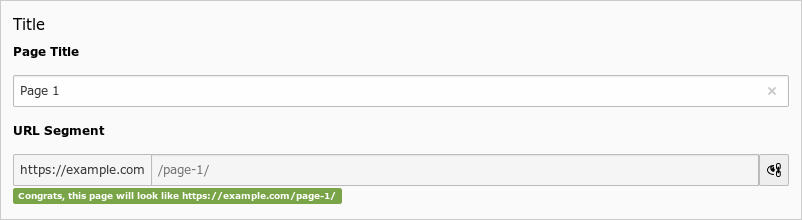
\includegraphics[width=0.8\linewidth]{PageBasedUrlHandling/UrlRouting.png}
	\end{figure}

%	\begin{figure}
%		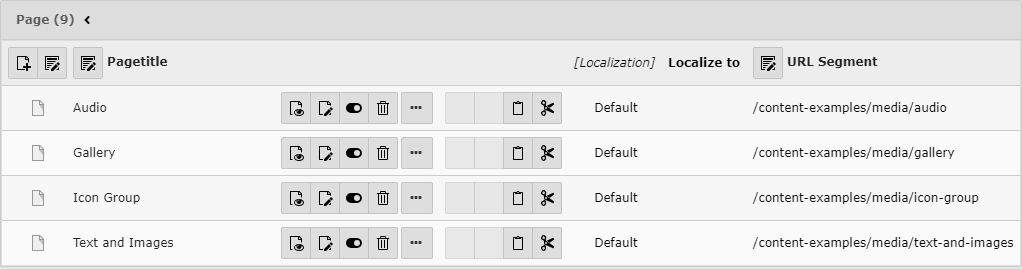
\includegraphics[width=0.8\linewidth]{PageBasedUrlHandling/85947-UrlSegments.png}
%	\end{figure}

\end{frame}

% ------------------------------------------------------------------------------
% #84729 - New TCA type "slug"

\begin{frame}[fragile]
	\frametitle{Seitenbasiertes URL-Handling}
	\framesubtitle{Neues TCA Feld \texttt{slug}}

	% decrease font size for code listing
	\lstset{basicstyle=\smaller\ttfamily}

	\begin{itemize}
		\item Ein neues TCA Feld \texttt{slug} wurde eingeführt
		\item Dies definiert teile eines URL-Pfades zum Generieren und Auflösen von URLs

		\begin{lstlisting}
'type' => 'slug',
  'config' => [
    'generatorOptions' => [
      'fields' => ['title', 'nav_title'],
      'fieldSeparator' => '/',
      'prefixParentPageSlug' => true
    ]
    'fallbackCharacter' => '-',
    'eval' => 'uniqueInSite'
  ]
		\end{lstlisting}
	\end{itemize}

\end{frame}

% ------------------------------------------------------------------------------
% #86365 - Routing Enhancers and Aspects

\begin{frame}[fragile]
	\frametitle{Seitenbasiertes URL-Handling}
	\framesubtitle{Routing "Enhancers" und "Aspects"}

	% decrease font size for code listing
	\lstset{basicstyle=\smaller\ttfamily}

	\begin{itemize}
		\item Routen können um "Platzhalter" erweitert werden, um einen URL-Pfad zu erstellen:
			\smaller\texttt{/path-to/my-page/products/\{product-name\}}\normalsize
		\item Das wird mit Hilfe von "Enhancers" und "Aspects" durchgeführt
		\item TYPO3 v9 LTS unterstützt die folgenden "Enhancers" out-of-the-box:

			\begin{itemize}
				\item Simple Enhancer (Enhancer Typ "Simple")
				\item Plugin Enhancer (Enhancer Typ "Plugin")
				\item Extbase Plugin Enhancer (Enhancer Typ "Extbase")
			\end{itemize}

		\item Die Konfiguration wird in der Datei \texttt{config.yml} gemacht
		\item Benutzerdefinierte Enhancer können in \texttt{ext\_localconf.php} registriert werden:

\begin{lstlisting}
$GLOBALS['TYPO3_CONF_VARS']['SYS']['routing']['CustomPlugin'] =
  \MyVendor\MyPackage\Routing\CustomEnhancer::class;
\end{lstlisting}
	\end{itemize}

\end{frame}

% ------------------------------------------------------------------------------
% #86160 - Add the possibility to use .html suffix in seo friendly URLs

\begin{frame}[fragile]
	\frametitle{Seitenbasiertes URL-Handling}
	\framesubtitle{Seitentyp Enhancer}

	% decrease font size for code listing
	\lstset{basicstyle=\smaller\ttfamily}

	\begin{itemize}
		\item Mit dem \texttt{PageTypeEnhancer} können Seiten nach deren Typ konfigueriert werden,
			z.B. die mit einem  \texttt{.html} Suffix
		\item Das Suffix wird am Ende einer URL mithilfe von
			\texttt{StaticValueMapper} hinzugefügt
		\item Konfigurationsbeispiel:

\begin{lstlisting}
routeEnhancers:
  PageType:
    type: PageType default: ''
	map:
	  '.html': 1
	  'menu.json': 13
\end{lstlisting}

	\end{itemize}

\end{frame}

% ------------------------------------------------------------------------------
